\documentclass[journal,12pt,twocolumn]{IEEEtran}

\usepackage{enumitem}
\usepackage{amsmath}
\usepackage{amssymb}
\usepackage{gensymb}
\usepackage{graphicx}
\usepackage{txfonts}         
\usepackage{listings}
\usepackage{lstautogobble}
\usepackage{mathtools}
\usepackage{bm}
\usepackage{hyperref}
\usepackage{polynom}
\usepackage{siunitx}
\usepackage{verbatim}

\newcommand{\solution}{\noindent \textbf{Solution: }}
\providecommand{\pr}[1]{\ensuremath{\Pr\left(#1\right)}}
\providecommand{\brak}[1]{\ensuremath{\left(#1\right)}}
\providecommand{\cbrak}[1]{\ensuremath{\left\{#1\right\}}}
\providecommand{\sbrak}[1]{\ensuremath{\left[#1\right]}}
\providecommand{\mean}[1]{E\left[ #1 \right]}
\providecommand{\var}[1]{\mathrm{Var}\left[ #1 \right]}
\providecommand{\der}[1]{\mathrm{d} #1}
\providecommand{\gauss}[2]{\mathcal{N}\ensuremath{\left(#1,#2\right)}}
\providecommand{\mbf}{\mathbf}
\providecommand{\abs}[1]{\left\vert#1\right\vert}
\providecommand{\norm}[1]{\left\lVert#1\right\rVert}
\providecommand{\z}[1]{{\mathcal{Z}}\cbrak{#1}}
\providecommand{\ztrans}{\overset{\mathcal{Z}}{ \rightleftharpoons}}

\providecommand{\parder}[2]{\frac{\partial}{\partial #2} \brak{#1}}

\let\StandardTheFigure\thefigure
\let\vec\mathbf

\numberwithin{equation}{section}
\renewcommand{\thefigure}{\theenumi}
\renewcommand\thesection{\arabic{section}}

\newcommand{\myvec}[1]{\ensuremath{\begin{pmatrix}#1\end{pmatrix}}}
\newcommand{\mymat}[1]{\ensuremath{\begin{bmatrix}#1\end{bmatrix}}}
\newcommand{\mydet}[1]{\ensuremath{\begin{vmatrix}#1\end{vmatrix}}}
\newcommand{\define}{\stackrel{\triangle}{=}}

\DeclareMathOperator*{\argmin}{arg\,min}
\DeclareMathOperator*{\argmax}{arg\,max}

\makeatletter
\def\pld@CF@loop#1+{%
    \ifx\relax#1\else
        \begingroup
          \pld@AccuSetX11%
          \def\pld@frac{{}{}}\let\pld@symbols\@empty\let\pld@vars\@empty
          \pld@false
          #1%
          \let\pld@temp\@empty
          \pld@AccuIfOne{}{\pld@AccuGet\pld@temp
                            \edef\pld@temp{\noexpand\pld@R\pld@temp}}%
           \pld@if \pld@Extend\pld@temp{\expandafter\pld@F\pld@frac}\fi
           \expandafter\pld@CF@loop@\pld@symbols\relax\@empty
           \expandafter\pld@CF@loop@\pld@vars\relax\@empty
           \ifx\@empty\pld@temp
               \def\pld@temp{\pld@R11}%
           \fi
          \global\let\@gtempa\pld@temp
        \endgroup
        \ifx\@empty\@gtempa\else
            \pld@ExtendPoly\pld@tempoly\@gtempa
        \fi
        \expandafter\pld@CF@loop
    \fi}
\def\pld@CMAddToTempoly{%
    \pld@AccuGet\pld@temp\edef\pld@temp{\noexpand\pld@R\pld@temp}%
    \pld@CondenseMonomials\pld@false\pld@symbols
    \ifx\pld@symbols\@empty \else
        \pld@ExtendPoly\pld@temp\pld@symbols
    \fi
    \ifx\pld@temp\@empty \else
        \pld@if
            \expandafter\pld@IfSum\expandafter{\pld@temp}%
                {\expandafter\def\expandafter\pld@temp\expandafter
                    {\expandafter\pld@F\expandafter{\pld@temp}{}}}%
                {}%
        \fi
        \pld@ExtendPoly\pld@tempoly\pld@temp
        \pld@Extend\pld@tempoly{\pld@monom}%
    \fi}
\makeatother

\lstset {
	frame=single, 
	breaklines=true,
	columns=fullflexible,
	autogobble=true
}             
                               
\title{Pingala Series \\ \Large EE3900: Linear Systems and Signal Processing \\ \large Indian Institute of Technology Hyderabad}
\author{Ankit Saha \\ \normalsize AI21BTECH11004 \\ \vspace*{20pt} \normalsize 28 Sep 2022}

\begin{document}

\maketitle

\section{JEE 2019}
Let 
\begin{align}
	a_n &= \frac{\alpha^{n}-\beta^{n}}{\alpha - \beta}, \quad n \ge 1
	\\
	b_n &= a_{n-1} + a_{n+1}, \quad n \ge 2, \quad b_1 =1
	\label{eq:10-orig-diff}
\end{align}
Verify the following using a python code.
\begin{enumerate}[label=\thesection.\arabic*,ref=\thesection.\theenumi]
\item 
\begin{align}
	\sum_{k=1}^{n}a_k = a_{n+2}-1, \quad n \ge 1
\end{align}
 \item 
\begin{align}
	\sum_{k=1}^{\infty}\frac{a_k}{10^k} =\frac{10}{89}
\end{align}
 \item 
\begin{align}
	b_n =\alpha^n + \beta^n, \quad n \ge 1
\end{align}
 \item 
\begin{align}
	\sum_{k=1}^{\infty}\frac{b_k}{10^k} =\frac{8}{89}
\end{align}
\end{enumerate}
\solution Download the following Python code that verifies the above
	\begin{lstlisting}
		wget https://github.com/Ankit-Saha-2003/EE3900/raw/main/Pingala/codes/1.py
	\end{lstlisting}
	
	Run the code by executing
	\begin{lstlisting}
		python 1.py
	\end{lstlisting}
	
	It turns out that everything apart from the last equation is true

\section{Pingala Series}
\begin{enumerate}[label=\thesection.\arabic*,ref=\thesection.\theenumi]
\item The {\em one sided} $Z$-transform of $x(n)$ is defined as 
\begin{align}
	X^{+}(z) = \sum_{n = 0}^{\infty}x(n)z^{-n}, \quad z \in \mathbb{C}
\label{eq:one-Z}
\end{align}
	\item The {\em Pingala} series is generated using the difference equation 
\begin{align}
	x(n+2) &= x\brak{n+1} + x\brak{n} \\  \quad x(0) &= x(1) = 1, n \ge 0
	\label{eq:10-pingala}
\end{align}
Generate a stem plot for $x(n)$.

\solution
Download the following Python code that plots Fig. \ref{fig-1}
\begin{lstlisting}
wget https://github.com/Ankit-Saha-2003/EE3900/raw/main/Pingala/codes/2.2.py
\end{lstlisting}

Run the code by executing
\begin{lstlisting}
python 2.2.py
\end{lstlisting}

\begin{figure}[!htp]
    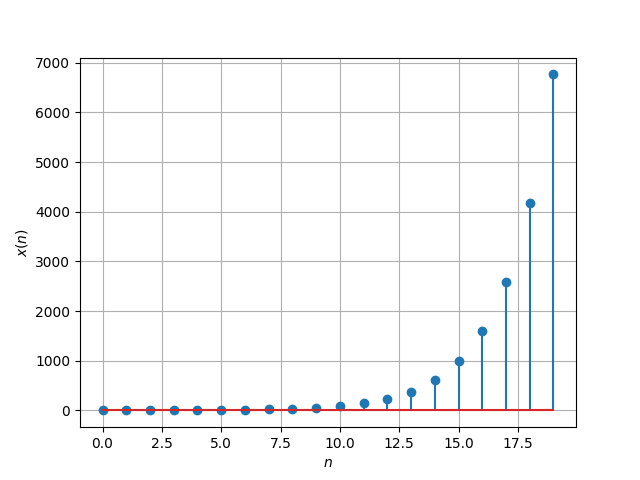
\includegraphics[width=\columnwidth]{figs/fig-1.png}
    \caption{Plot of $x(n)$}
    \label{fig-1}
\end{figure}


\newpage
\item Find $X^{+}(z)$

\solution 

We have
\begin{equation}
	x(n+2) = x(n+1) + x(n) \qquad n \ge 0
\end{equation}

On taking the one-sided $Z$-transform on both sides of the equation, we get
\begin{align}
	\mathcal{Z}^+\cbrak{x(n+2)} = \mathcal{Z}^+\cbrak{x(n+1) + x(n)}
\end{align}

Since, the one-sided $Z$-transform is a linear transformation
\begin{align}
    \implies &\mathcal{Z}^+\cbrak{x(n + 2)} = \mathcal{Z}^+\cbrak{x(n + 1)} + \mathcal{Z}^+\cbrak{x(n)} \\
    \implies &\sum_{n=0}^\infty x(n+2)z^{-n} = \sum_{n=0}^\infty x(n+1)z^{-n} + \sum_{n=0}^\infty x(n)z^{-n} 
\end{align}

But
\begin{align}
	\sum_{n=0}^\infty x(n+2)z^{-n} &= z^2 \sum_{k=2}^\infty x(k) z^{-k} \\
	&= z^2 \brak{X^+(z) - x(0) - x(1) z^{-1}} \\
	&= z^2 X^+(z) - z^2 - z \\
	\sum_{n=0}^\infty x(n+1)z^{-n} &= z \sum_{k=1}^\infty x(k) z^{-k} \\
	&= z \brak{X^+(z) - x(0)} \\
	&= z X^+(z) - z
\end{align}

Thus
\begin{align}
    \implies&z^2X^+(z) - z^2 - z = zX^+(z) - z + X^+(z) \\
    \implies&\brak{z^2 - z - 1}X^+(z) = z^2 \\
    \implies&X^+(z) = \frac{1}{1 - z^{-1} - z^{-2}} \\
    \therefore&X^+(z) = \frac{1}{\brak{1 - \alpha z^{-1}}\brak{1 - \beta z^{-1}}} \quad |z| > \max\brak{\abs{\alpha}, \abs{\beta}}
\end{align}

\item Find $x(n)$

\solution Using partial fraction decomposition
\begin{align}
	X^+(z) &= \frac{1}{\brak{\alpha - \beta}z^{-1}}\brak{\frac{1}{1 - \alpha z^{-1}} - \frac{1}{1 - \beta z^{-1}}}
\end{align}

We know that
\begin{align}
	\frac{1}{1 - \alpha z^{-1}} &\ztrans \alpha^n u(n) \\
	\frac{1}{1 - \beta z^{-1}} &\ztrans \beta^n u(n) \\
	zF(z) &\ztrans f(n+1)
\end{align}

Since we are dealing with the unit step function here, the $Z$-transform and the one-sded $Z$-transform are both the same
\begin{align}
	x(n) = \frac{1}{\alpha - \beta}  \brak{\alpha^{n+1} u(n+1) - \beta^{n+1} u(n+1)}
\end{align}

Since at $n=-1$, $x(n)$ is zero anyway, we can write
\begin{align}
	x(n) = \frac{\alpha^{n+1} - \beta^{n+1}}{\alpha - \beta} u(n)
\end{align}

	\item Sketch 
\begin{align}
	y(n) = x\brak{n-1} + x\brak{n+1}  \quad n \ge 0
	\label{eq:10-orig-diff-rev}
\end{align}

\solution
Download the following Python code that plots Fig. \ref{fig-2}
\begin{lstlisting}
wget https://github.com/Ankit-Saha-2003/EE3900/raw/main/Pingala/codes/2.5.py
\end{lstlisting}

Run the code by executing
\begin{lstlisting}
python 2.5.py
\end{lstlisting}

\begin{figure}[!htp]
    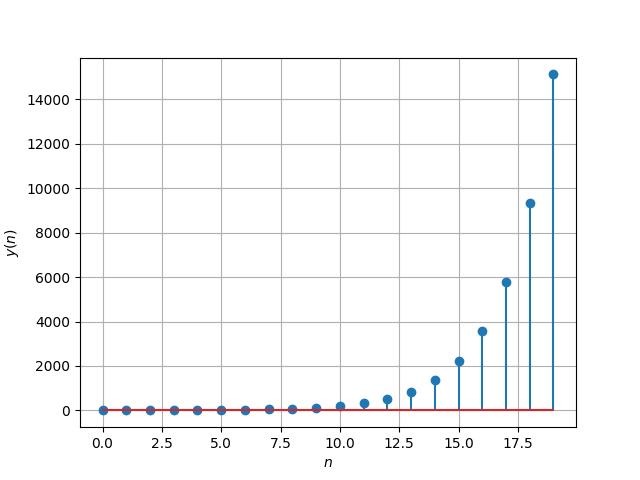
\includegraphics[width=\columnwidth]{figs/fig-2.png}
    \caption{Plot of $y(n)$}
    \label{fig-2}
\end{figure}

\item Find $Y^{+}(z)$

\solution We have
\begin{equation}
	y(n) = x(n-1) + x(n+1) \quad n \ge 0
\end{equation}

On taking the one-sided $Z$-transform on both sides of the equation, we get
\begin{align}
\mathcal{Z}^+\cbrak{y(n)} &= \mathcal{Z}^+\cbrak{x(n-1) + x(n+1)} \\
 &= \mathcal{Z}^+\cbrak{x(n + 1)} + \mathcal{Z}^+\cbrak{x(n - 1)} \\
 &= \sum_{n=0}^\infty x(n+1)z^{-n} + \sum_{n=0}^\infty x(n-1)z^{-n}
\end{align}

But
\begin{align}
	\sum_{n=0}^\infty x(n-1)z^{-n} &= z^{-1}\sum_{k=-1}^\infty x(k)z^{-k} \\
	&= z^{-1} \brak{X^+(z) + x(-1)z} \\
	&= z^{-1} X^+(z)
\end{align}

Thus
\begin{align}
Y^+(z) &= zX^+(z) - z + z^{-1}X^+(z)  \\
&= \frac{z + z^{-1}}{1 - z^{-1} - z^{-2}} - z \\
&= \frac{z + z^{-1} - z + 1 + z^{-1}}{1 - z^{-1} - z^{-2}} \\
&= \frac{1 + 2z^{-1}}{1 - z^{-1} - z^{-2}} \qquad |z| > \max\brak{\abs{\alpha}, \abs{\beta}}
\end{align}

\item Find $y(n)$

\solution 
\begin{align}
	y(n) &= x(n+1) + x(n-1) \quad n \ge 0 \\
	&= \frac{\alpha^{n+2} - \beta^{n+2}}{\alpha - \beta} u(n+1) + \frac{\alpha^{n} - \beta^{n}}{\alpha - \beta} u(n-1)
\end{align}

We have
\begin{align}
	y(n) &= 0 \qquad \forall n < 0 \\
	y(0) &= x(1) + x(-1) = 1 + 0 = 1
\end{align}

For $n > 0$
\begin{align}
	y(n) &= \frac{\alpha^{n+2} - \beta^{n+2} + \alpha^{n} - \beta^{n}}{\alpha - \beta}
\end{align}

Since $\alpha\beta = -1$
\begin{align}
	y(n) &= \frac{\alpha^{n+2} -(\alpha\beta)\alpha^{n} - \beta^{n+2}  + (\alpha\beta)\beta^{n}}{\alpha - \beta} \\
	&= \frac{\alpha^{n+1}(\alpha - \beta) + \beta^{n+1}(\alpha - \beta)}{\alpha - \beta} \\
	&= \alpha^{n+1} + \beta^{n+1}
\end{align}

If we plug in $n=0$ in this equation, we get
\begin{equation}
	y(0) = \alpha + \beta = 1
\end{equation}
which is consistent with what we obtained earlier

Therefore
\begin{equation}
	y(n) = (\alpha^{n+1} + \beta^{n+1})u(n)
\end{equation}


\end{enumerate}

\section{Power of the Z transform}
\begin{enumerate}[label=\thesection.\arabic*,ref=\thesection.\theenumi]
\item Show that 
\begin{align}
	\sum_{k=1}^{n}a_k = 
	\sum_{k=0}^{n-1}x(k) = x(n)*u(n-1)
\end{align}

\solution We have obtained that $a_n = x(n-1)$
\begin{align}
	\sum_{k=1}^{n}a_k &= \sum_{k=1}^n x(k-1) \\
	&= \sum_{k=0}^{n-1} x(k)
\end{align}

Also
\begin{align}
	x(k) &= 
	\begin{cases}
		1 & k \ge 0 \\
		0 & k < 0
	\end{cases} \\
	u(n-1-k) &=
	\begin{cases}
		1 & k \le n - 1 \\
		0 & k > n - 1
	\end{cases}
\end{align}

Thus
\begin{align}
	\sum_{k=0}^{n-1} x(k) &= \sum_{k=-\infty}^{\infty} x(k) u(n-1-k) \\
	&= x(n)*u(n-1)
\end{align}

\item Show that 
\begin{align}
a_{n+2}-1 \qquad n \ge 1
\end{align}
can be expressed as 
\begin{align}
	(x(n+1) - 1)u(n)
\end{align}

\solution 
\begin{align}
a_{n+2}-1 \qquad n \ge 1
\end{align}
can be written as
\begin{align}
(a_{n+2}-1) u(n-1)
\end{align}

Since the system defined by $a$ is time-invariant and $a_n$ is just $x(n)$ shifted forward by one unit, we can shift this backward by one unit to get the expression in terms of $x$
\begin{align}
	a_{n+2} &\rightleftharpoons x(n+1) \\
	u(n-1) &\rightleftharpoons u(n)
\end{align}

Therefore, the above expression can be expressed as
\begin{align}
	(x(n+1) - 1)u(n)
\end{align}

\item Show that 
\begin{align}
	\sum_{k=1}^{\infty}\frac{a_k}{10^k}= 
	\frac{1}{10}\sum_{k=0}^{\infty}\frac{x\brak{k}}{10^k} =\frac{1}{10}X^{+}\brak{{10}}
\end{align}

\solution 
\begin{align}
    \sum_{k=1}^{\infty}\frac{a_k}{10^k} 
    &= \sum_{k = 0}^{\infty}\frac{a_{k+1}}{10^{k+1}} && k \rightarrow k + 1 \\
    &= \frac{1}{10}\sum_{k = 0}^{\infty}\frac{a_{k+1}}{10^k} \\
    &= \frac{1}{10}\sum_{k = 0}^{\infty}\frac{x(k)}{10^k} &&\because a_{k+1} = x(k) \\
    &= \frac{1}{10}\sum_{k = 0}^{\infty} x(k) 10^{-k} \\
    &= \frac{1}{10}X^+(10) 
\end{align}

\item Show that 
\begin{align}
	\alpha^n + \beta^n \qquad n \ge 1
\end{align}
can be expressed as 
\begin{align}
	w(n) = \brak{\alpha^{n+1} + \beta^{n+1}}u(n)
\end{align}
and find $W(z)$

\solution 
\begin{align}
	\alpha^n + \beta^n \qquad n \ge 1
\end{align}
can be written as
\begin{align}
	(\alpha^n + \beta^n) u(n-1)
\end{align}

On shifiting this backward by one unit, we get
\begin{align}
	(\alpha^{n+1} + \beta^{n+1}) u(n)
\end{align}
by time-invariance

Now
\begin{align}
	w(n) &= \alpha \cdot \alpha^n u(n) + \beta \cdot \beta^n u(n) 
\end{align}

We know that
\begin{align}
	\alpha^n u(n) &\ztrans \frac{1}{1-\alpha z^{-1}} &&\abs{z} > \abs{\alpha} \\
	\beta^n u(n) &\ztrans \frac{1}{1-\beta z^{-1}} &&\abs{z} > \abs{\beta}
\end{align}

Therefore
\begin{align}
	W(z) &= \frac{\alpha}{1-\alpha z^{-1}} + \frac{\beta}{1-\beta z^{-1}} &&\abs{z}>\max(\abs{\alpha}, \abs{\beta}) \\
	&= \frac{\alpha(1-\beta z^{-1}) + \beta(1-\alpha z^{-1})}{(1-\alpha z^{-1})(1-\beta z^{-1})} \\
	&= \frac{\alpha + \beta  - 2\alpha\beta z^{-1}}{1 - (\alpha + \beta)z^{-1} + \alpha\beta z^{-2}} \\
	&= \frac{1 + 2z^{-1}}{1 - z^{-1} - z^{-2}}
\end{align}


 \item Show that 
\begin{align}
	\sum_{k=1}^{\infty}\frac{b_k}{10^k} =
	\frac{1}{10}\sum_{k=0}^{\infty}\frac{y\brak{k}}{10^k} =\frac{1}{10}Y^{+}\brak{{10}}
\end{align}

\solution Note that
\begin{align}
	b_n &= a_{n-1} + a_{n+1} && n \ge 2, ~b_1 =1 \\
	&= x(n-2) + x(n) \\
	&= y(n-1) && n \ge 2
\end{align}

At $n=1$, $y(0) = 1$ anyway, thus
\begin{align}
	b_n = y(n-1) \qquad n \ge 1
\end{align}

Now
\begin{align}
    \sum_{k=1}^{\infty}\frac{b_k}{10^k} 
    &= \sum_{k = 0}^{\infty}\frac{b_{k+1}}{10^{k+1}} && k \rightarrow k + 1 \\
    &= \frac{1}{10}\sum_{k = 0}^{\infty}\frac{b_{k+1}}{10^k} \\
    &= \frac{1}{10}\sum_{k = 0}^{\infty}\frac{y(k)}{10^k} &&\because b_{k+1} = y(k) \\
    &= \frac{1}{10}\sum_{k = 0}^{\infty} y(k) 10^{-k} \\
    &= \frac{1}{10}Y^+(10) 
\end{align}

\item Solve the JEE 2019 problem.

\solution We have shown that
\begin{align}
    \sum_{k = 1}^{n}a_k = x(n)*u(n - 1)
\end{align}

On taking the $Z$-transform on both sides of the equation
\begin{align}
    \z{\sum_{k = 1}^{n}a_k} &= X(z) \brak{z^{-1} U(z)} \\
    &= \frac{z^{-1}}{\brak{1 - z^{-1} - z^{-2}}\brak{1 - z^{-1}}} \\
    &= \frac{1}{z^{-1}}\brak{\frac{1}{1 - z^{-1} - z^{-2}} - \frac{1}{1 - z^{-1}}} 
\end{align}

On taking the inverse $Z$-transform on both sides of this equation, we get
\begin{align}
    \sum_{k = 1}^{n}a_k &= x(n+1)u(n) - u(n+1)
\end{align}

For $n \ge 1$
\begin{align}
	\sum_{k = 1}^{n}a_k &= x(n+1) - 1 \\
	&= a_{n+2} - 1 && n \ge 1
\end{align}

We have proved that
\begin{align}
	\sum_{k=1}^\infty \frac{a_k}{10^k} &= \frac{1}{10} X^+(10) \\
	&= \frac{1}{10} \frac{1}{(1 - 10^{-1} - 10^{-2})} \\
	&= \frac{1}{10} \frac{100}{100 - 10 - 1} \\
	&= \frac{10}{89}
\end{align}

We have also shown that
\begin{align}
	b_n = y(n-1) \qquad n \ge 1
\end{align}

But
\begin{align}
	y(n) = (\alpha^{n+1} + \beta^{n+1})u(n)
\end{align}

Thus
\begin{align}
	b_n &= (\alpha^n + \beta^n)u(n-1) && n \ge 1 \\
	&= \alpha^n + \beta^n && n \ge 1
\end{align}

We have also proved that
\begin{align}
	\sum_{k=1}^\infty \frac{b_k}{10^k} &= \frac{1}{10} Y^+(10) \\
	&= \frac{1}{10} \frac{1 + 2(10)^{-1}}{(1 - 10^{-1} - 10^{-2})} \\
	&= \frac{1}{10} \frac{100 + 20}{100 - 10 - 1} \\
	&= \frac{12}{89}
\end{align}

Therefore, all of the options except the last option are correct
\end{enumerate}
\end{document}
